\section{Wireless Sensor Networks}\label{s:WirelessSensorNetworks}

Der Begriff 'Wireless Sensor Network' bezeichnet eine Ansammlung von Sensoren, welche miteinander kommunzieren und bestimmte Zustände der Umwelt erfassen und analysieren. In den folgenden Unterkapiteln werden wichtige Aspekte, welche die WSNs auszeichnet, aufgezeigt.

\subsection{Ubiquit\"ares Rechnen}\label{ss:UbiquitaeresRechnen}

1988 verwendete Mark Weiser erstmals den Begriff 'ubiquitous computing' (dt. ubiquitäres Rechnen), um seine Vision nach einem stets verfügbaren Rechensystem, welches dem Nutzer unsichtbar erscheinen soll, zum Ausdruck zu bringen. Der Computer soll sich so in den Alltag integrieren, dass die Menschen ihn gar nicht mehr bemerken. Nach seiner Vorstellung verbessere das ubiquitäre Rechnen die Erfahrungen, die man mit Computern macht, da die Rechner dem Nutzer nahtlos verfügbar gemacht werden, ohne dabei effektiv sichtbar zu sein.\\

Weiser zufolge sind die besten Technologien diejenigen, die scheinbar verschwinden, tatsächlich jedoch nur in den Hintergrund geraten und unsichtbar werden. Der Mensch soll nicht in der Welt des Computers leben, sondern der Rechner soll sich in die Welt des Menschen integrieren. In Lichtschaltern, Thermostaten, Stereoanlagen und Backöfen werden bereits heute kleine Rechner verbaut, die helfen sollen, den Alltag zu erleichtern und die Idee des 'Internet of Things' weiter zu verfolgen.\\

Da Ubiquitäres Rechnen zuverlässig und unsichtbar funktionieren soll, ist die Technologie der unsichtbaren Rechenmodule von großer Bedeutung. Voraussetzungen sind z.B. leistungsstarke Prozessoren, ausreichend Speicherplatz, drahtlose Kommunikation sowie Sensoren und Aktoren (die z.B. mit der Umwelt und dem Menschen interagieren). Der Mensch muss nicht für alle Anwendungsfälle von ubiquitärem Rechnen direkt eingebunden werden, da die Systeme auch autonom arbeiten können\cite{d:wolf}.\\
\subsection{Motivation von Sensornetzen}\label{ss:MotivationSensornetze}

Sensornetze sind sehr flexibel und können unter anderem dafür eingesetzt werden, um
\begin{itemize}
	\item Umwelteinflüsse wahrzunehmen ('sensing')
	\item Umwelteinflüsse zu verarbeiten und zu analysieren ('computing')
	\item Daten zu übertragen ('transport')
	\item Netzwerke für verteile Systeme aufzubauen ('networking')
	\item Die Umwelt zu beeinflussen und zu verändern ('actuation')
\end{itemize}

F\"ur viele Anwendungsfälle und Szenarien, in denen mit der Umwelt interagiert wird, soll die Benutzung von drahtlosen Sensornetzen zukünftig ausgebaut und etabliert werden. Der Einsatz von Sensornetzen kann dabei verschiedene Motivationen und Anforderungen haben:
\begin{itemize}
	\item Direkte Interaktion mit Menschen ist nicht möglich oder nicht erforderlich (z.B. bei Überwachung einer Maschine in der Industrie)
	\item Der Mensch soll nur im Notfall alarmiert werden (z.B. in Notfällen oder wenn die Sensoren bestimmte Schwellenwerte erreichen)
	\item Es handelt sich um ein autonomes System, welches nur Selten das Handeln eines Menschen erfordert
\end{itemize}

\begin{figure}[H] 
	\centering
	
\includegraphics[scale=0.5]{Bilder/mooreslaw}
	\caption{Mikroprozessoren-Transistoren im Laufe der Zeit\cite{i:mooreslaw}}
	\label{f:mooreslaw}
\end{figure}

Eine weitere Motivation der Verwirklichung von drahtlosen Sensornetzen ist der Technologiefortschritt, der es möglich macht, immer kleinere Rechengeräte herzustellen und miteinander zu vernetzen. Um diesen Fortschritt zu verdeutlichen, formulierte Gordon Moore 1965 ein Gesetz, welches besagt, dass sich die Anzahl der integrierten Schaltkreise auf einem Mikroprozessor alle 18-24 Monate verdoppelt \cite{d:wolf}. \\

MOORES LAW weiter erläutern und Bild hier noch einfügen

\subsection{Bestandteile}\label{ss:Bestandteile}
\subsection{Topologien}\label{ss:Topologien}

Bei einem Aufbau eines Sensornetzes stellt sich grundsätzlich die Frage, wie die einzelnen Sensoren miteinander Verbindungen aufbauen und kommunizieren sollen. Ein solche Verbindungsstruktur nennt sich in der Informatik 'Topologie'. Da das Sensornetz insgesamt zuverlässig arbeiten soll, Kosten und Komplexität jedoch gering gehalten werden sollen, wurden speziell für die drahtlosen Sensornetze neue Ansätze im Bereich der Topologie erforscht. Im folgenden sollen 4 Topologie-Alternativen näher erläutert werden. \\

Peer-to-Peer Netzwerke erlauben es, das jeder Knoten im Netz (in unserem Fall der Sensor) mit jedem anderen Knoten direkt Kontakt aufnehmen kann. Jedes 'Peer-Gerät' ist gleichzeitig Client und Server gegenüber anderen Knoten im Netzwerk.\\

\begin{figure}[H] 
	\centering
	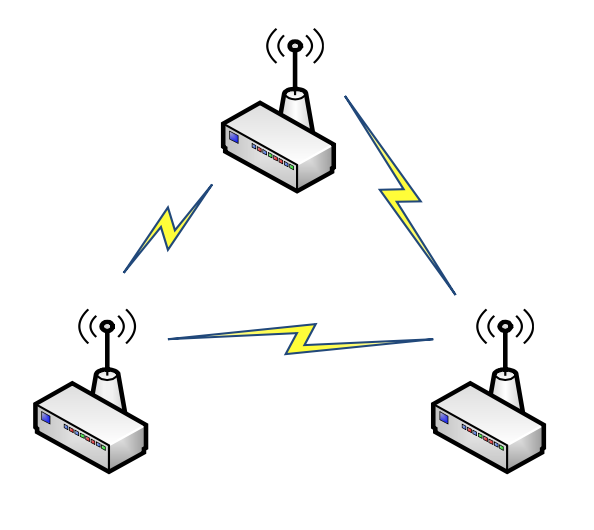
\includegraphics[scale=0.5]{Bilder/peertopeer}
	\caption{Peer-To-Peer Netzwerk\cite{d:kosmerchock}}
	\label{f:peertopeer}
\end{figure}

Bei der Stern-Topologie sind die Sensoren an ein zentrales Kommunikationsgerät angebunden. In diesem Fall kommunizieren die einzelnen Knoten nicht direkt miteinander. Jegliche Art von Kommunikation wird über das zentrale Gerät (auch Hub genannt) geroutet. Der Hub wird hier als Server betrachtet, wohingegen die Knoten (Sensoren) die Clients darstellen. \\

\begin{figure}[H] 
	\centering
	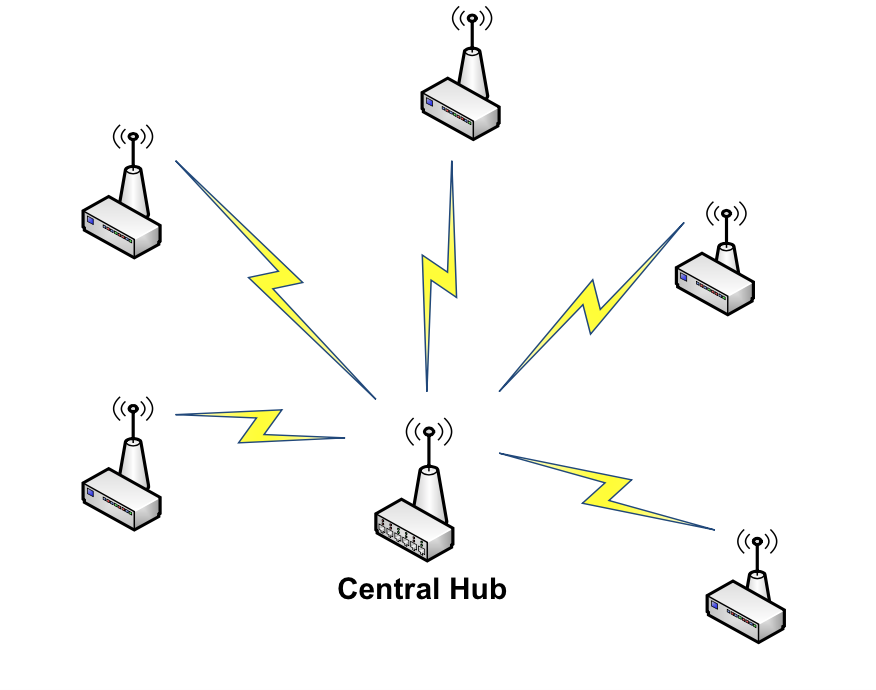
\includegraphics[scale=0.5]{Bilder/star}
	\caption{Stern Netzwerk\cite{d:kosmerchock}}
	\label{f:star}
\end{figure}

Die Baum-Topologie stellt eine Hybridvariante aus Peer-to-Peer und Stern dar. Sie nutzt einen sogenannten 'Root-Knoten' als zentraler Router. Eine Ebene darunter liegen die Hubs, an denen wie in der Stern-Topologie die Sensoren angebunden sind. \\

\begin{figure}[H] 
	\centering
	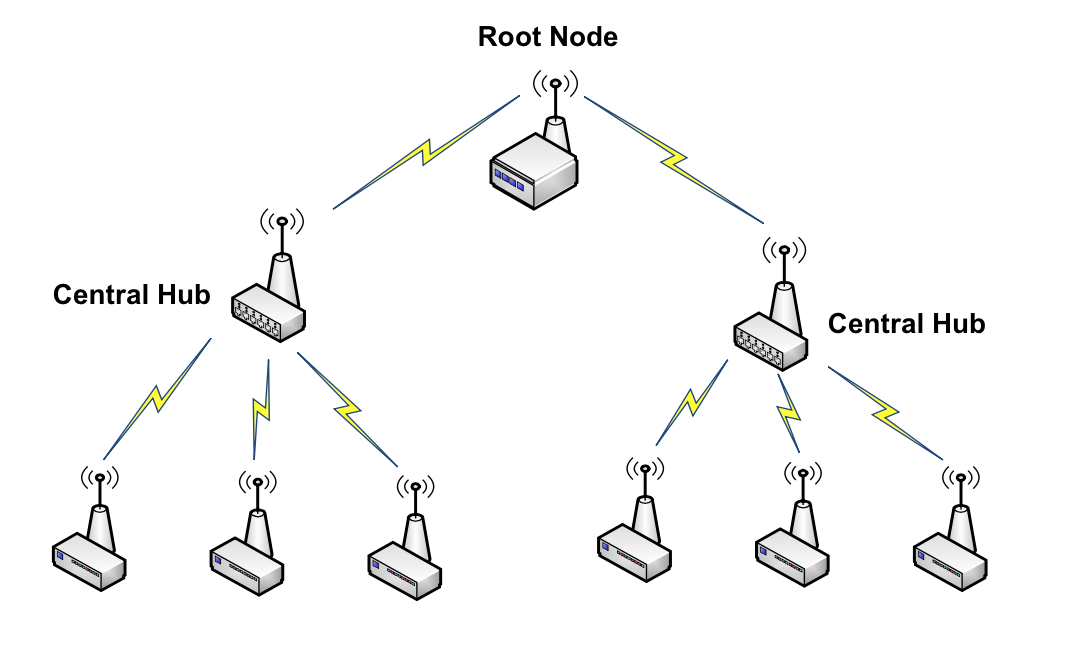
\includegraphics[scale=0.5]{Bilder/tree}
	\caption{Baum Netzwerk\cite{d:kosmerchock}}
	\label{f:tree}
\end{figure}

Eine weitere Mögliche Variante ist ein vermaschtes Netz. Die Knoten sind untereinander ohne zentralen Hub verbunden und die Daten werden einfach von Knoten zu Knoten weitergesendet, bis sie ihr gewünschtes Ziel erreicht haben \cite{d:kosmerchock}. 

\begin{figure}[H] 
	\centering
	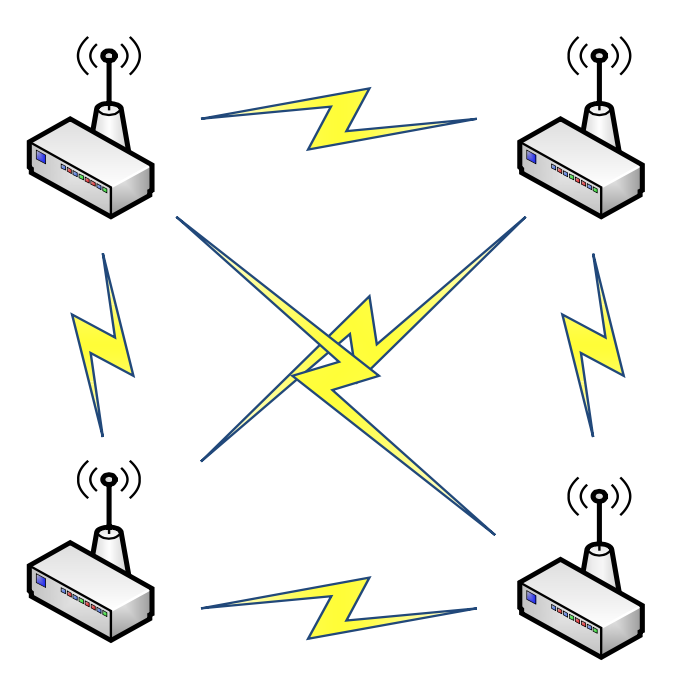
\includegraphics[scale=0.5]{Bilder/mesh}
	\caption{Vermaschtes Netzwerk\cite{d:kosmerchock}}
	\label{f:mesh}
\end{figure}
\subsection{Schwierigkeiten}\label{ss:Schwierigkeiten}

Beim Planen eines drahtlosen Sensornetzwerkes stellen sich vermehrt einige Schwierigkeiten heraus, die zu berücksichtigen sind. Viele dieser Schwierigkeiten sind auch untereinander abhängig und beeinflussen gleichzeitig die verwendete Elektronik, physikalische Aspekte, Rechenleistung oder auch Lebensdauer eines Sensors.\\

Die erste Schwierigkeit, die es bei einem Sensor zu betrachten gilt, ist die Versorgung des Sensors mit Energie. Dazu gibt es unterschiedliche Ansätze, wie z.B. die Versorgung des Sensors mit Batterien. Dies hat allerdings den Nachteil, dass deren Lebenszyklus beschränkt ist und Batterien früher oder später ausgetauscht werden müssen. Ein Akkumulator eignet sich hier besser, allerdings bleibt die Frage, wie der Akkumulator mit neuem Strom versorgt werden soll.\\

In Zusammenhang mit dieser Fragestellung ist die Betrachtung der möglichen Gewinnung oder Rückgewinnung von Energie durch den Sensor von Vorteil. Wie kann ein Sensor Energie gewinnen, ohne dass er damit direkt versorgt werden muss? Möglichkeiten wäre die Gewinnung von Solarenergie durch den Sensor, das Nutzen von Temperaturunterschieden in der Umwelt, die Rückgewinnung der Bewegungsenergie (z.B. durch Wind o.ä.) oder das Ausnutzen von Erschütterungen und Vibrationen. Diese Möglichkeiten sollten nur in Betracht gezogen werden, wenn der Sensor eine lange Lebensdauer mit sich bringen soll. Ist der Einsatz der Sensoren in absehbarer Zeit vorüber, lohnt es sich aus Produktions- und Kostengründen die begrenzte Lebenszeit des Sensors hinzunehmen, um ihn danach z.B. durch neue Sensoren auszutauschen.\\

Ein weiterer wichtiger Aspekt im Bereich Energie ist die Energieeffizienz. Dabei sollen alle Teile in einem Sensorknoten möglichst effizient arbeiten, um die Energie sinnvoll und langsam aufzubrauchen. Nicht nur der Sensor selbst spielt dabei eine wichtige Rolle, sondern auch wie das Netzwerk um ihn herum aufgebaut und genutzt wird. Folgende Aspekte spielen bei der Energieeffizienz eine erhebliche Rolle:

\begin{itemize}
	\item Wahrnehmen der Daten durch die Sensoren
	\item Verarbeitung der Daten
	\item Sicherung der Daten
	\item Übertragung der Daten
	\item Empfang von Daten
\end{itemize} 
\newpage
Damit der Energieverbrauch weiter eingeschränkt werden kann, sollten Sensoren nur aktiv sein, wenn sie wirklich benötigt werden. Ansonsten sollten sie sich in einen Sleep- bzw. Energiesparmodus begeben, um Energie zu sparen. Des Weiteren wäre zur ausschließlichen Wahrnehmung der Umgebung ein 'Controller'- bzw. Sensormodus und zum Senden und Empfangen von Daten ein 'Radio'- bzw. Übertragungsmodus von Vorteil.\\

Eine weitere Schwierigkeit, die sich stellt, ist der Einsatz bzw. die Verteilung der Sensoren in der Umwelt und ihre Selbstverwaltung. Die Knoten könnten entweder zufällig in der Umgebung platziert oder systematisch angeordnet werden. Hier entscheidet der jeweilige Anwendungszweck, wobei das systematische Platzieren der Sensoren meistens sinnvoller und effizienter ist.
Des Weiteren sollte unterschieden werden, ob aktive oder passive Sensoren eingesetzt werden sollen. Auch hier muss je nach Anwendungsfall unterschieden werden. Passive Sensoren eignen sich besser, wenn Daten nur erfasst und übermittelt werden sollen. Aktive Sensoren sollten eingesetzt werden, wenn auf die Erfassung der Daten eine eventuelle Aktion bzw. Reaktion mit der Umwelt erforderlich ist.\\ 

Sensoren sollten bestimmte Informationen über sich selbst und ihre Nachbarn wissen bzw. ermitteln können. Dazu gehören unter anderem ihre eigene Position, die Ortung der Nachbarknoten und ihre Identifikation, ihre eigene Knotenkonfiguration und ihre kürzeste Route zu einer Basisstation. Denn sobald ein Sensornetz einmal in Betrieb genommen wurde, muss es in der Lage sein, sich autonom betreiben und verwalten zu können. Dazu zählen die Anpassung an veränderte Umweltbedingung und das Kompensieren von Fehlern. Beim Ausfall eines einzelnen Sensors soll das Sensornetz weiterhin aktiv und funktionsfähig bleiben.\\

Auch in Hinsicht auf die Sicherheit gibt es einige Aspekte zu betrachten. Manche Sensornetzwerke übertragen empfindliche und kritische Informationen, was sie zu einem beliebten Angriffsziel macht. Sie können sowohl von innen, von außen als auch direkt an den Knoten angegriffen werden. Es stellt sich als schwierig heraus, solche Netzwerke vor Angriffen zu schützen, da sie entfernt und selbstständig arbeiten, drahtlos kommunizieren und meistens keine speziellen Sicherheitsfeatures besitzen. Dies ist aus Energie-, Kostengründen und Gründen der Form und Größe der Sensoren meist nicht realisierbar. Übliche Sicherheitstechniken sind meist nicht durchführbar, da den Knoten üblicherweise die Rechen-, Kommunikations- und Speicherressourcen fehlen. Man braucht neu entwickelte Sicherheitsmechanismen für Sensornetze, die spezielle Lösungen für die Erkennung von Eindringlingen, Verschlüsselung, Schlüsselverwaltung und Verteilung und Registrierung von neuen Knoten besitzen, sodass die Ressourcen der Sensoren ausreichen und das Sicherheitskonzept realisierbar ist \cite{d:wolf}.
\section{Adhoc-Netzwerke}\label{s:AdhocNetzwerke}

Adhoc-Netze sind in sich geschlossene Netzwerke, organisieren sich selbst und haben keine bestimmte Hierarchie. Sie bauen sich nur für die Dauer einer Datenübertragung auf, besitzen keine festgelegte Kommunikationsstruktur und verwalten und organiseren sich selbst. 

Adhoc-Netze sind leistungsfähige und zählen als so genanntes 'Self Organized Network' (SON), welche gute Lastverteilung betreiben und ohne zentrales Management auskommen. Die Endgeräte übernehmen in diesem Fall das Routing und speichern die Routingtabellen selbst ab. Geräte, die sich dem Netzwerk anschließen, werden dynamisch in das Netz eingefügt. Bei Netzwerken nach IEEE 802.11 (WLANs) und IEEE 802.15 (WPANs - hier im Speziellen IEEE 802.15.1 - Bluetooth) werden alle Geräte selbstständig erkannt und werden dem Netz hinzugefügt. Sie sind fortan Bestandteil des Gesamtnetzes. 

Bei Adhoc-Netzen mit vielen Geräten (das kann z.B. ein Sensornetz sein) wird zumeist eine Multihop-Verbindung bevorzugt. Das bedeutet, dass die Daten von einem Netzknoten, z.B. einem Sensor oder Rechner, zu dem nächsten Netzknoten weitergeleitet werden, bis es sein Ziel erreicht hat. Fällt ein Knoten aus, wird wenn möglich ein anderer Weg für die Übertragung genutzt, um Ausfälle zu vermeiden.

Ad-hoc-Netzwerke bestehen virtuell für einen begrenzten Zeitrahmen. Ad-hoc bedeutet etwa "für den Augenblick gemacht". Sie werden in WLANs, WPANs, in Sensornetzen (WPANs mit geringer Datenrate - siehe IEEE 802.15.4) und in Funknetzen von Rettungsdiensten, Polizei und Militär benutzt \cite{ws:lipinski}.

\subsection{MANETs}\label{ss:MANETs}

MANET bezeichnet die Abkürzung für den Begriff 'Mobile Ad-hoc Network‘. Jochen Schiller beschreibt in seiner Literatur 'Mobile Communications' den Begriff des MANETs wie folgt:
 
\begin{quote}
„Ad-hoc-Netze kommen ohne jegliche Infrastruktur aus, insbesondere ohne eine ausgezeichnete Basisstation, welche den Medienzugriff zentral steuert. Diese Netzvariante erlaubt die spontane, nicht vorab geplante Kommunikation zwischen mobilen Endgeräten, wobei einige oder alle Endgeräte auch Daten von anderen Endgeräten weiterleiten können.“
\end{quote}
	
\begin{figure}[H] 
	\centering
	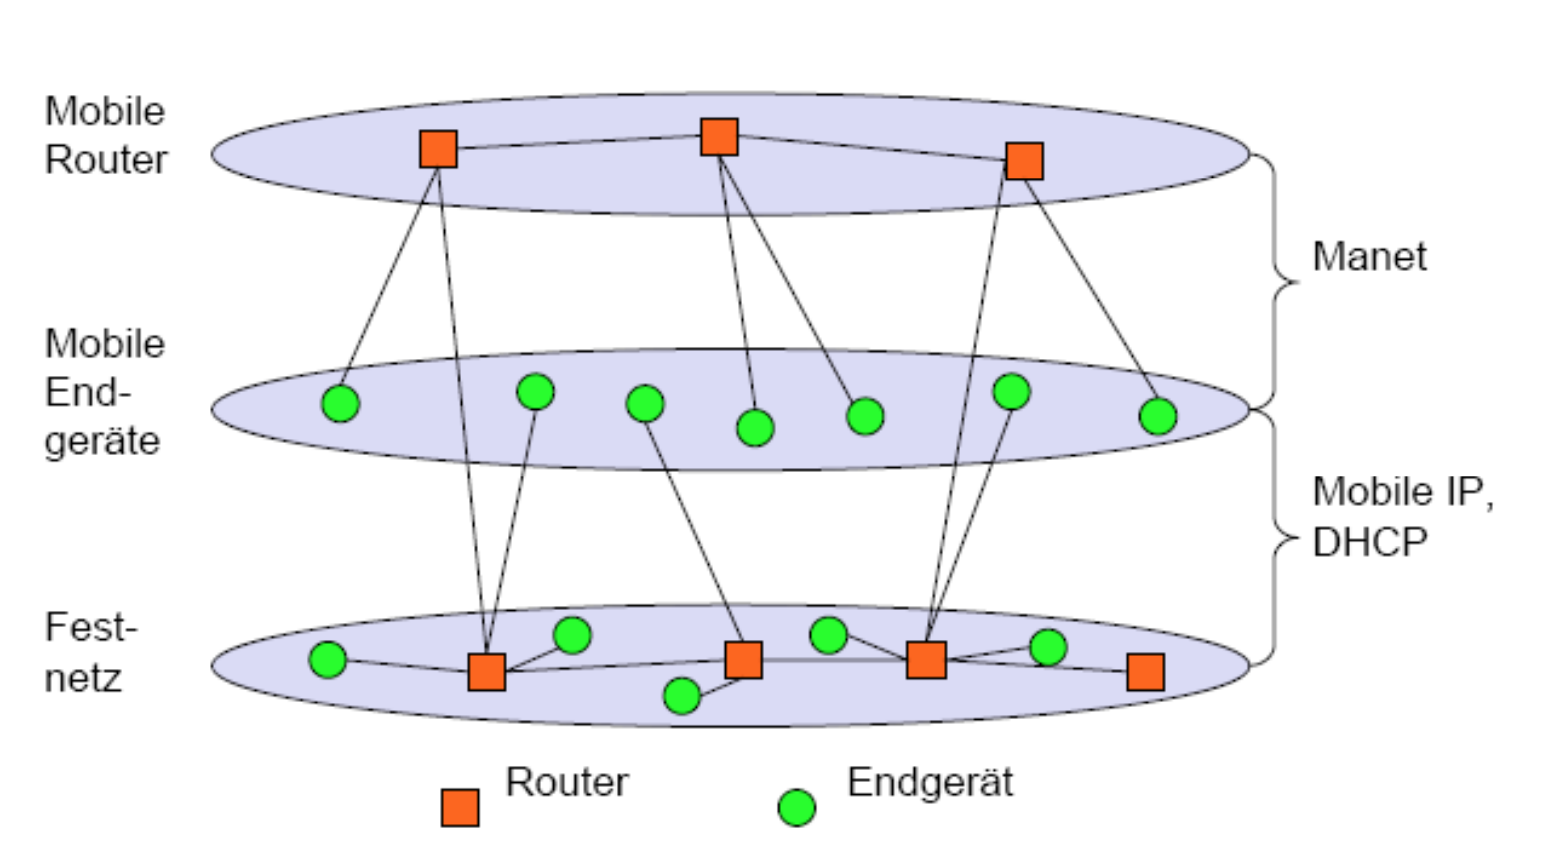
\includegraphics[scale=0.5]{Bilder/manet}
	\caption{Einordnung von MANETs\cite{d:timm}}
	\label{f:manet}
\end{figure}

MANETs zeichnen sich vor allem dadurch aus, dass sie keine feste Infrastruktur besitzen. Es herrscht innerhalb des Netzes eine dynamische Topologie, was bedeutet, dass zu jedem Zeitpunkt bestimmte Knoten wegfallen und neue dazukommen können. Dies führt dazu, dass bislang bekannte und zulässige Routen wegfallen, dafür aber auch neue Routen entstehen können. Unter den Geräten besteht eine spontane Vernetzung. Das bedeutet, dass jedes Gerät sowohl Endpunkt einer Übertragung sein kann, jedoch auch in der Lage sein muss, Daten weiterleiten zu können. Durch dieses Weiterleiten von Daten entsteht eine so genannte 'Multihop-Umgebung‘, da die Daten nicht vom Sender direkt zum Empfänger gelangen, sondern den Empfänger über mehrere Zwischenstationen erreichen. \\

\begin{figure}[H] 
	\centering
	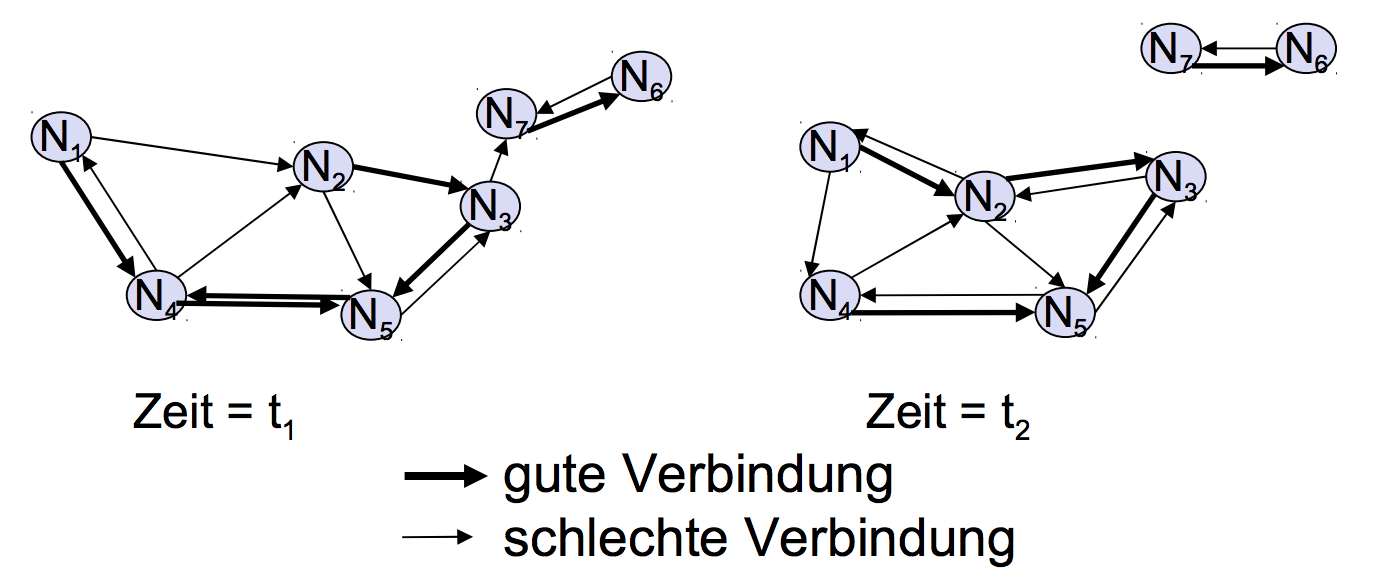
\includegraphics[scale=0.5]{Bilder/manetconnection}
	\caption{Mögliche Verbindungen eines Beispiel MANETs\cite{d:timm}}
	\label{f:manetconnection}
\end{figure}

Mobile Ad-hoc Netzwerke besitzen eine stark begrenzte Bandbreite. Da sie meistens auf stromsparende Übertragungsprotokolle setzen, können dementsprechend auch nur geringe Mengen an Daten übertragen werden. Des Weiteren bestehen zumeist durch die unterschiedlichen Übertragungsleistungen der Geräte asymmetrische Verbindungen, welche sich für die Übertragung von Daten innerhalb des Netzes besser eignen.\\

Ein Problem bei MANETs stellt die beschränkte Möglichkeit der Energieversorgung dar, da die Endgeräte meistens abhängig von Batterien oder Akkus sind. Durch die hohe Menge an Geräten in einem Netz steigt dazu die Summe des potenziellen Energiebedarfes pro Gerät weiter an. Auch die Sicherung des Netzes vor physischen Angriffen ist stark beschränkt. So sind z.B. Denial-of-Service-Attacken (DoS), Überwachungsangriffe oder auch das Verfälschen von Nachrichten oft leicht zu realisieren \cite{d:timm}.

\subsection{Routingprotokolle}\label{ss:Routingprotokolle}

Klassische Routingprotokolle versagen bei dem Versuch, sie innerhalb von mobilen Ad-hoc Netzwerken einzusetzen. Gründe dafür sind folgende: \\

MANETs zeichnen sich durch eine hohe Dynamik aus, das Netz verändert sich spontan, schnell und ständig. Klassische Protokolle besitzen eine zu langsame Konvergenz, um dem Anspruch der sich ständig verändernden Ad-hoc Netze gerecht zu werden und sind somit nicht geeignet.\\

Ad-hoc Netze besitzen wie bereits erwähnt meist eine geringe Bandbreite. Hinzu kommt, dass den angeschlossenen Knoten und Geräten nur eine gewisse Rechenleistung zur Verfügung steht. Sie sind somit mit klassischen Routingprotokollen überfordert, da diese meist viel Rechenleistung und Übertragungsleistung erfordern, welche mit den mobilen Geräten nicht realisierbar sind. Der Overhead der klassischen Protokolle ist also für diese Art von Netzwerken zu groß. \\

Es gibt in mobilen Ad-hoc Netzen gewisse Metriken, die beim Betrieb berücksichtigt werden müssen. Die klassischen Protokolle interessieren sich nicht für diese Metriken und lassen sie außen vor. Bei der Auswahl von Routen müssen unter anderem folgende Aspekte betrachtet werden:
\begin{itemize}
	\item Batterielaufzeit der Geräte
	\item Zeit der Verbindung zwischen zwei Geräten
	\item Energiebedarf
	\item Zuverlässigkeit der Verbindung
\end{itemize} 

Zusammengefasst lässt sich sagen, dass Routingprotokolle für MANETs vor allem eine große Skalierbarkeit im Hinsicht auf eine große Anzahl von Geräten, Flexibilität und Effizienz im Hinblick auf Komplexität, Energieverbrauch und Speicherverbrauch erfordern. Diese werden mittlerweile intensiv erforscht, da Ad-hoc Netze im Zusammenhang mit dem 'Internet of Things‘ (IoT) oder auch dem 'Internet Of Everything‘ (IoE) zunehmend an Bedeutung gewinnen \cite{d:timm}. \\

Im Folgenden sollen die Protokolle OLSR, AODV und CGSR kurz aufgezeigt und erklärt werden.

\subsubsection{OLSR}\label{ss:OLSR}

Die Abkürzung OLSR steht für 'Optimized Link State Routing‘ und bezeichnet ein flaches, proaktives Linkstate-Protokoll. Proaktiv bedeutet in diesem Fall, dass in gewissen Zeitabständen automatisch Kontrollnachrichten ausgetauscht werden. Bei einem Linkstate-Protokoll sendet z.B. jeder Router den anderen Knoten im Netz den Zustand der Verbindung zu seinen Nachbarn. \\
Das OLSR-Routingprotokoll ist als RFC 3626 spezifiziert und erweitert normale Link-State-Protokolle, in dem die Komplexität jener Protokolle vereinfacht wird. \\
Bei OLSR hat jeder Knoten einen Überblick über alle andere Knoten im Netzwerk und den Routen dort hin, somit kann jeder Knoten seine Routen mit dem 'Shortest Path Algorithm‘ eigenständig errechnen. Allerdings haben nicht alle Knoten die gleichen Bedeutungen und Aufgaben.\\
Um Nachbarknoten zu finden, werden sie mit einer 'Hello-Message‘ gesucht. Die Kontrollpakete werden in entsprechenden Zeitabständen erstellt und enthalten die Knotenadresse, eine Sequenznummer und die Nachbarknoten mit Distanzinformationen. Folglich enthält jeder Knoten die Distanzinformationen von allen anderen Knoten, so kann die Topologie erstellt und die Routen mit o.g. 'Shortest Path Algorithm‘ berechnet werden. \\

Das OLSR unterscheidet sich von anderen Link-State-Algorithmen, da es ein optimiertest Link-State-Routing verwendet. Es werden so genannte 'Multi-Point-Relays‘ ausgewählt und verteilt, was für ein effizienteres Routing sorgt. Die Relays sind im Stande, die Kontrollnachrichten an die angeschlossenen Knoten weiterzuleiten.

\begin{figure}[H] 
	\centering
	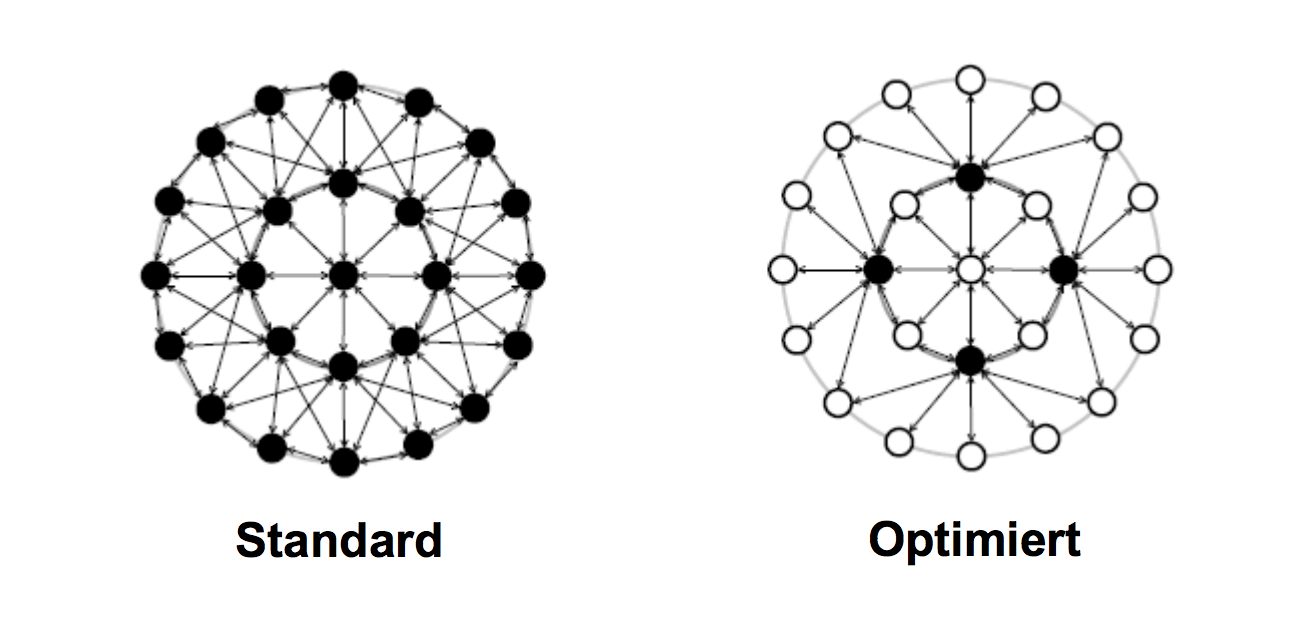
\includegraphics[scale=0.5]{Bilder/olsr}
	\caption{optimiertes LSR durch Multi-Point-Relays im OLSR\cite{d:timm}}
	\label{f:olsr}
\end{figure}

\subsubsection{AODV}\label{ss:AODV}

Das Ad-hoc On-Demand Distance Vector Routingprotokoll ist ein flaches, reaktives Distanzvektorprotokoll. Reaktive Protokolle tauschen im Gegensatz zu proaktiven Protokollen nur Kontrollnachrichten aus, wenn neue Routen benutzt werden sollen. Sie benötigen weniger Bandbreite und sind dynamischer, allerdings besteht nur eine Teilkenntnis des Netzwerks, somit müssen die Routen anders berechnet werden.\\
AODV ist in RFC 3561 spezifiziert und ist für IPv4-Netze vorgesehen. Es erlaubt eine theoretisch unbegrenzte Anzahl von Geräten im Netzwerk. Bei AODV  kennt jeder Knoten nur den 'Next Hop‘, also den nächsten Knoten und die Länge der Gesamtroute. Das Protokoll definiert insgesamt zwei Routingalgorithmen ‚Route Discovery‘ und ‚Route Maintenance‘.  \\

Bei der 'Route Discovery‘ wird die Route aufgebaut, wozu zwei Nachrichtentypen benötigt werden. Es wird zunächst eine 'Route-Request-Nachricht‘ (RREQ) per Broadcast zum Ziel gesendet. Das Ziel antwortet widerum mit einer 'Route-Reply-Nachricht‘ (RREP) per Unicast zurück an den Absender. Sollte eine bidirektionale Verbindung zwischen zwei Geräten herrschen, wird per Route Discovery auch eine bidirektionale Route aufgebaut. \\

\begin{figure}[H] 
	\centering
	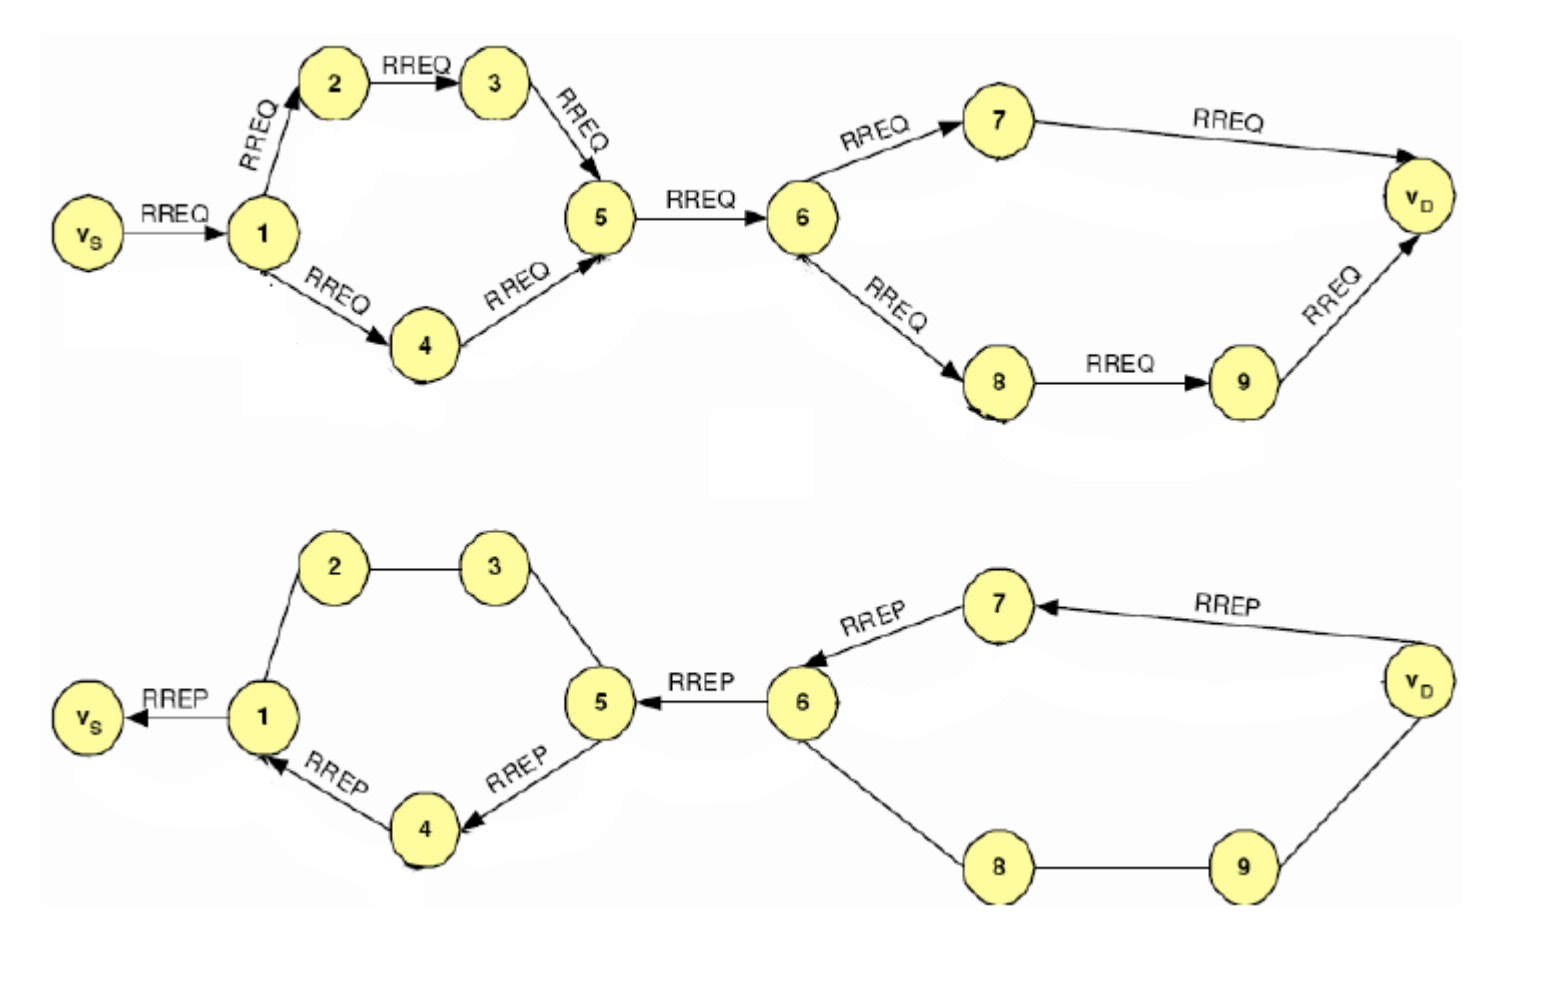
\includegraphics[scale=0.5]{Bilder/aodv}
	\caption{'Route Discovery‘ im AODV-Protokoll\cite{d:timm}}
	\label{f:aodv}
\end{figure}

Bei 'Route Maintenance‘ handelt es sich um die Verwaltung der Routen. Es wird eine 'Route-Error-Nachricht‘ (RRER) versendet, sobald eine defekte Route diagnostiziert wird. Diese Nachricht wird an alle Nachbarn versendet, so dass jeder Knoten über das Wegfallen der Route informiert wird.

\subsubsection{CGSR}\label{ss:CGSR}

Beim Clusterhead-Gateway Switch Routing (CGSR) handelt es sich um ein hierarchisches Protokoll, was bedeutet, dass für verschiedene Knoten unterschiedliche Rollen vorgesehen sind. \\
Das Netzwerk wird bei CGSR in Cluster aufgeteilt, die sich allerdings teilweise überdecken müssen. Für jedes dieser Cluster wird ein 'Clusterhead‘ ernannt. Ein Knoten, welcher sich in zwei Clustern gleichzeitig befindet, wird als Gateway bezeichnet.

\begin{figure}[H] 
	\centering
	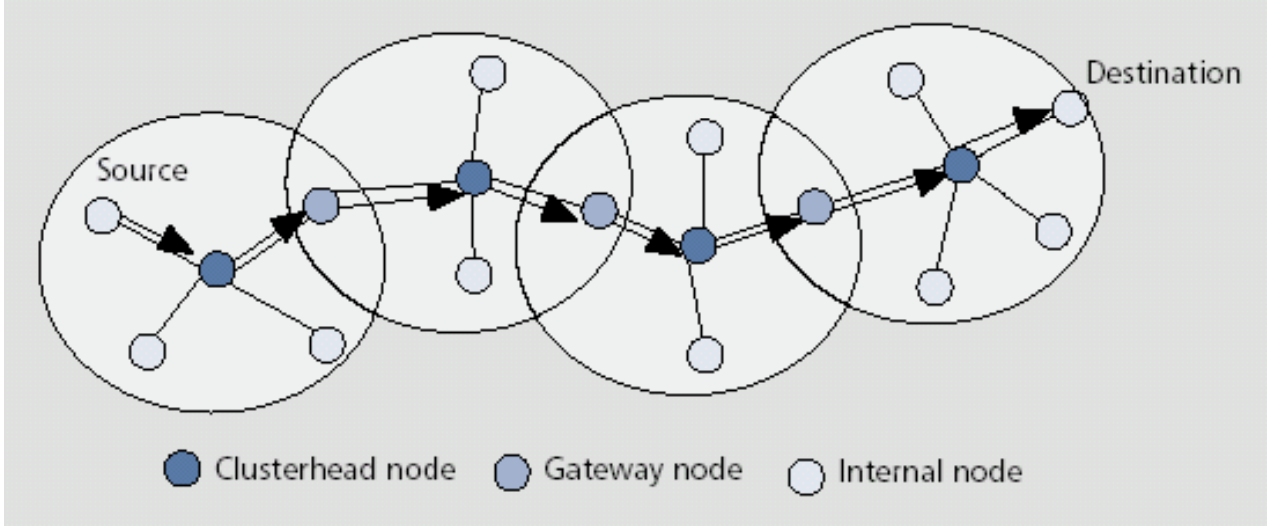
\includegraphics[scale=0.5]{Bilder/cgsr}
	\caption{Clustering im CGSR-Protokoll\cite{d:timm}}
	\label{f:cgsr}
\end{figure}

Das Clusterhead-Gateway Switch Routing basiert auf einem Distanzvektor-Protokoll. Jeder Knoten im Netzwerk speichert sowohl eine Distanzvektor-Routingtabelle, als auch eine 'Cluster Member‘-Tabelle. Die Distanzvektor-Tabelle enthält neben den normalen Routingeinträgen einen Routingeintrag zum Clusterhead jedes Clusters. In der 'Cluster Member‘-Tabelle wird für jeden Knoten der Clusterhead gespeichert, damit klar ist, welcher Knoten zu welchem Cluster gehört. \\

Der große Vorteil von CGSR besteht in der signifikanten Reduzierung der Größe der Routingtabellen im Vergleich zu anderen Distanzvektorprotokollen, somit ist das CGSR für Ad-hoc Netzwerke dank seiner geringeren Komplexität gut geeignet.


\section{IEEE 802.15.4}\label{ss:IEEE802154}

Das ‚Institute of Electrical and Electronics Engineers‘ (IEEE) definiert in seinem Standard 802.15.4 Protokolle für ein ‚Low Data Rate - Wireless Personal Area Network‘ (LR-WPAN). Die Art der Geräte, die für eine solche Art von Netz verwendet werden sollen, ist dabei nicht genauer spezifiziert. Sinnvoll ist der Einsatz vor allem bei Systemen wie Sensoren, Lichtquellen oder Schaltern, bei welchen eine niedrige Datenrate vollkommen ausreicht um miteinander zu kommunizieren. Grundsätzlich ist die Verwendung des Standards auch bei höherwertigen Geräten wie z.B. Handys oder anderen Multimediageräten möglich, allerdings ist die Sinnhaftigkeit eines solchen Einsatzes fragwürdig, da in Hinsicht auf die geringe Datenübertragungsrate viele Übertragungs- und Kommunikationsfunktionen solcher Geräte wohl kaum realisierbar wären. \\
Zur Kommunikation mehrerer Teilnehmer in einem nach 802.15.4-standardisierten Netzes werden die o.g. Topologien ‚Stern‘ und ‚Peer-to-Peer‘ unterstützt. Sollte die Spezifikation ‚ZigBee‘,  welche den 802.15.4 Standard erweitert, verwendet werden, können darüber hinaus auch vermaschte Netze realisiert werden. \\
Der Standard sendet laut Definition festgelegtem Frequenzspektrum auf den lizenzfreien Frequenzen 868-868,8 MHz (Europa), 902-928 MHz (Nordamerika, Australien) oder 2400 bis 2483,5 MHz (weltweit). Um die Frequenzen darüber hinaus zu spreizen, wird ein ‚Direct Sequence Spread Spectrum‘-Verfahren (DSSS) verwendet. //
Um den Zugriff auf das Medium untereinander zu koordinieren, wird CSMA/CA (‚Carrier Sense Multiple Access/Collision Avoidance‘) verwendet. Das bedeutet, dass, bevor ein Gerät mit einer Übertragung beginnt, überprüft wird, ob das Übertragungsmedium nicht bereits von einem anderen Endgerät genutzt wird. Ist das Medium nicht belegt, kann das Endgerät, welches das Medium überprüft hat, anfangen, seine Daten zu übertragen.\\
Der Standard erreicht Übertragungsraten zwischen 20 KB/s - 40 KB/s in den Frequenzbereichen von 868 MHz und 902-928 MHz, wohingegen im 2,4 GHz-Bereich Raten bis zu 250 KB/s realisiert werden können. Diese relativ geringen Datenraten zeigen bereits, dass der Standard nicht für eine Übertragung großer Daten konzipiert wurde. Es soll viel mehr eine energiesparende Übertragung geringer Datenmengen verwirklicht werden können \cite{d:hesse}.

\subsection{Komponenten}\label{ss:Komponenten}

\subsection{Unterstützte Topologien}\label{ss:UnterstutzeTopologien}

\subsection{Schichten}\label{ss:Schichten}

\subsection{Rahmenstruktur}\label{ss:Rahmenstruktur}

\subsection{Kommunikation}\label{ss:Kommunikation}

\subsection{Medienzugriff}\label{ss:Medienzugriff}

\subsection{Sicherheitsma"snahmen}\label{ss:Sicherheitsmassnahmen}